\chapter{Porównanie wydajności baz relacyjnych i nierelacyjnych}

W poprzednich rozdziałach skupiliśmy się na porównaniu czysto teoretycznym oraz praktycznym. W tym rozdziale poruszymy rzeczywiste różnice po zaimplementowaniu dwóch rozwiązań w jednym projekcie. Obie bazy danych są postawione na zewnętrznym serwerze, opóźnienia połączenia w obu przypadkach są porównywalne, więc skupmy się na czasie odpytywania.

\section{Wnioski z analizy czasu wyszukiwania między bazami}
Przy blisko pięćdziesięciu próbach wykres prezentuje się następująco:
\begin{figure}[h]
    \centering
    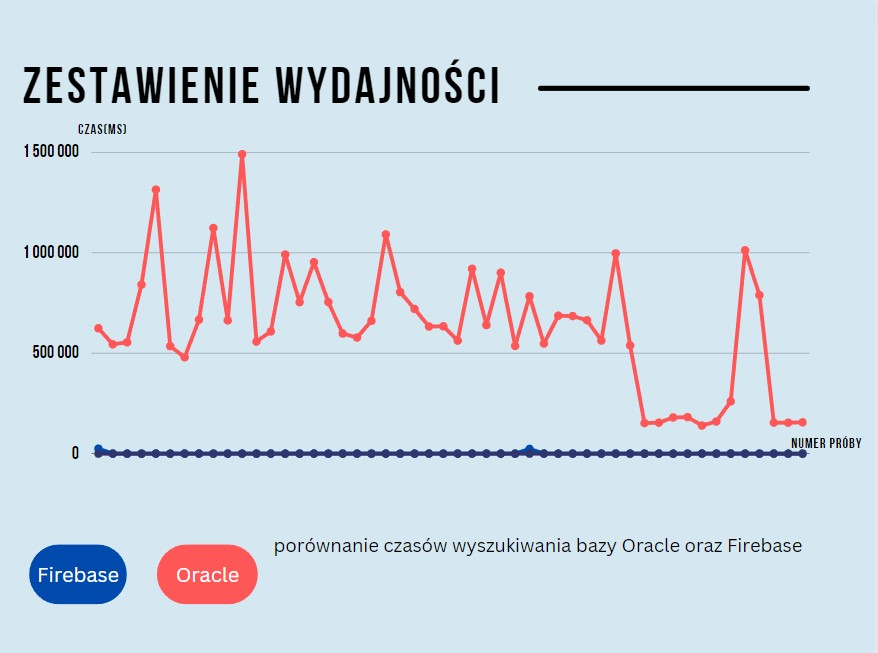
\includegraphics[width=1\linewidth]{./img/wykres.jpg}
    \caption{Wykres przedstawiający czas zapytania w milisekundach dla każdej próby}
    \label{fig:Wykres}
\end{figure}

Dane do powyższego wykresu, zostały pobrane z tabeli \textit{SEARCHING} opisanej w poprzednim rozdziale. Na osi Y widzimy czas w milisekundach potrzebny do pobrania wszystkich rekordów z bazy danych oraz przefiltrowania ich wobec preferencji użytkownika i zwróceniu do wyświetlenia użytkownikowi. Jak widzimy na powyższym wykresie różnica w wydajności działania bazy danych Firebase nad bazą danych Oracle jest miażdżąca. Z tej różnicy możemy wyciągnąć wniosek, iż Firebase jest wydajniejszy i bardziej przyszłościowy w stosunku do bazy relacyjnej Oracle.

Bazy nierelacyjne cechują się ogromną wydajnością i prędkością przeszukiwania, nie występuje tam tabelaryzacja jak po stronie baz relacyjnych, co ułatwia strukturę. Dla programistów implementacja jest dużo prostsza, bo wymaga tylko jednego serwisu do dodawania, usuwania oraz przeszukiwania rekordów, natomiast dla bazy relacyjnej potrzebujemy budować konkretne zapytania, jeśli mamy więcej warunków do wyszukiwania. Na przykładzie aplikacji \textit{FindYourGame} stworzonej w celu porównania baz relacyjnych i nierelacyjnych na przykładzie Firebase oraz Oracle database, dochodzimy do wniosku iż baza danych Firebase jest około 10000 razy wydajniejsza.


